\section{Method}\label{sec:method}

\subsection{Task Definition}

The target task is request-level web threat triage in a distributed defense system. Given an observed request $r$, the system must emit a handling decision $d \in \{\texttt{allow}, \texttt{monitor}, \texttt{challenge}, \texttt{block}\}$, together with a confidence-bearing rationale that can be reviewed later. The core object is not a single label, but a structured decision package:
\[
\mathcal{Y}(r) = \langle \mathbf{p}, d, \tau, \kappa \rangle
\]
where $\mathbf{p}$ is the final verdict distribution over \texttt{safe}, \texttt{suspicious}, and \texttt{malicious}; $\tau$ is the debate transcript; and $\kappa$ is the resulting case file.

Table~\ref{tab:symbols} defines the main symbols and interfaces used in the remainder of the paper. The formulation matches the repository implementation, in which each role emits a verdict distribution and the orchestration layer computes disagreement statistics before deciding whether debate is necessary.

\begin{table}[t]
  \centering
  \caption{Core symbols and operational objects.}
  \label{tab:symbols}
  \begin{tabular}{p{0.14\columnwidth}p{0.78\columnwidth}}
    \toprule
    Symbol & Meaning \\
    \midrule
    $r$ & observed web request with path, headers, body, and source metadata \\
    $\mathcal{A}$ & role set \{Socrates, Plato, Aristotle\} \\
    $\mathbf{p}_i$ & role-specific verdict distribution over \{safe, suspicious, malicious\} \\
    $c_i$ & role-specific confidence score \\
    $\delta(r)$ & disagreement state computed from role outputs \\
    $\tau$ & debate transcript generated only when disagreement is material \\
    $\kappa$ & case file containing verdict, rationale, evidence summary, and follow-up action \\
    $m$ & routing mode from \{cloud\_only, local\_preferred, hybrid\_verify\} \\
    \bottomrule
  \end{tabular}
\end{table}

\subsection{Three-Role Debate Pipeline}

The method uses three fixed roles rather than a larger open-ended agent society. This is deliberate. In security operations, excess agent diversity can add verbosity without improving actionability. The three roles used here correspond to common operational viewpoints:
\begin{itemize}
  \item \textbf{Socrates}: adversarial challenge. This role assumes the request may be a bypass attempt or an underestimated attack mutation.
  \item \textbf{Plato}: defensive handling. This role reasons about response feasibility, policy consequences, and whether the evidence justifies intervention.
  \item \textbf{Aristotle}: synthesis and arbitration. This role aggregates the other views and is responsible for final verdict formation.
\end{itemize}

Each role emits an initial tuple $\langle \mathbf{p}_i, c_i, e_i \rangle$ containing a verdict distribution, a confidence score, and supporting evidence fragments. The first-stage result is therefore a set of parallel opinions rather than a single score.

\subsection{Debate Triggering}

Debate is not unconditional. It is only invoked when disagreement indicators suggest that the request is ambiguous enough to deserve explicit role conflict resolution. The trigger state is computed from three signals already present in the implementation:
\begin{enumerate}
  \item \textbf{label conflict}: whether the dominant labels of the role distributions differ;
  \item \textbf{distribution divergence}: the average pairwise Jensen--Shannon divergence across $\mathbf{p}_i$;
  \item \textbf{confidence range}: $\max_i c_i - \min_i c_i$.
\end{enumerate}

Let $\tau_d$ and $\tau_c$ denote divergence and confidence thresholds. Debate is triggered when
\begin{equation}
\begin{aligned}
\delta(r) = &\ \mathbb{I}[\text{label conflict}] \\
& \lor \mathbb{I}[\mathrm{JSD}_{avg}(\mathbf{p}_1,\mathbf{p}_2,\mathbf{p}_3) > \tau_d] \\
& \lor \mathbb{I}[\max_i c_i - \min_i c_i > \tau_c].
\end{aligned}
\end{equation}
This matches the repository scoring logic and intentionally focuses debate on hard cases instead of easy consensus cases.

\begin{figure}[t]
  \centering
  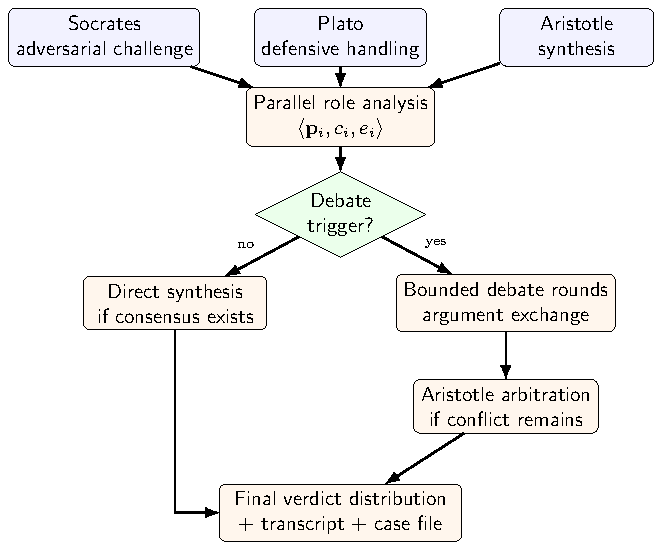
\includegraphics[width=\linewidth]{fig-debate-flow.pdf}
  \caption{Decision flow of the three-role debate pipeline.}
  \label{fig:debate-flow}
\end{figure}

\subsection{Arbitration and Auditable Outputs}

When debate is triggered, the three roles enter bounded rounds of argument exchange. The implementation uses a small maximum round budget and then falls back to Aristotle arbitration. This keeps the pipeline operationally predictable. The final verdict is produced by blending role distributions into an aggregate distribution $\bar{\mathbf{p}}$, from which the dominant label and confidence are extracted. Unlike a plain majority vote, the aggregate preserves uncertainty shape and can therefore distinguish between strong malicious consensus and weak suspicious consensus.

The crucial design choice is that the method outputs more than $d$. It emits three auditable products:
\begin{itemize}
  \item the \textbf{debate transcript}, which records why disagreement existed;
  \item the \textbf{final verdict distribution}, which records the shape of remaining uncertainty;
  \item the \textbf{case file}, which records the rationale and recommended follow-up action.
\end{itemize}
These artifacts operationalize ``explainability'' as traceable decision workflow rather than as feature attribution.

\subsection{Algorithm Sketch}

\begin{algorithm}[t]
  \caption{Debate-driven triage for request $r$}
  \label{alg:triage}
  \begin{algorithmic}[1]
    \Require observed request $r$, route mode $m$, role set $\mathcal{A}$
    \ForAll{$a_i \in \mathcal{A}$}
      \State compute initial role output $\langle \mathbf{p}_i, c_i, e_i \rangle$
    \EndFor
    \State compute disagreement state $\delta(r)$
    \If{$\delta(r)$ is true}
      \State execute bounded debate rounds
      \State let Aristotle arbitrate unresolved conflict
    \EndIf
    \State blend role distributions into $\bar{\mathbf{p}}$
    \State derive final handling decision $d$
    \State synthesize transcript $\tau$ and case file $\kappa$
    \State \Return $\langle \bar{\mathbf{p}}, d, \tau, \kappa \rangle$
  \end{algorithmic}
\end{algorithm}

Algorithm~\ref{alg:triage} highlights the paper's main methodological claim: explicit disagreement handling is the mechanism under study. The distributed platform, routing layer, and gateway security measures are implementation support that make this mechanism usable in practice.
